\section{TX}
\label{sec:tx}
\textit{\hyperlink{schematic.5}{schematic}}

\subsection{Overview}
\label{sec:tx-overview}

An RF frequency synthesizer and external VCO are used to generate a sine wave that is periodically
ramped from $5.3 \si{GHz}$ to $5.9 \si{GHz}$ over $1 \si{ms}$ with a $2 \si{ms}$ delay between
ramps. The signal is then power-amplified and a portion of the resulting signal is sent to an SMA
connector for transmission via an antenna and the remainder is kept on the board for mixing with the
received signal. Most of the power is directed for transmission.

\subsection{ADF4158 Frequency Synthesizer}
\label{sec:adf4158}

\subsubsection{Description}
\label{sec:adf4158-description}

The \href{http://www.analog.com/media/en/technical-documentation/data-sheets/ADF4158.pdf}{ADF4158}
is a 6.1GHz fractional-n frequency synthesizer. A block diagram describing its functionality is shown in
Figure~\ref{fig:adf4158-block-diagram}.

\begin{figure}[h]
        \centering
        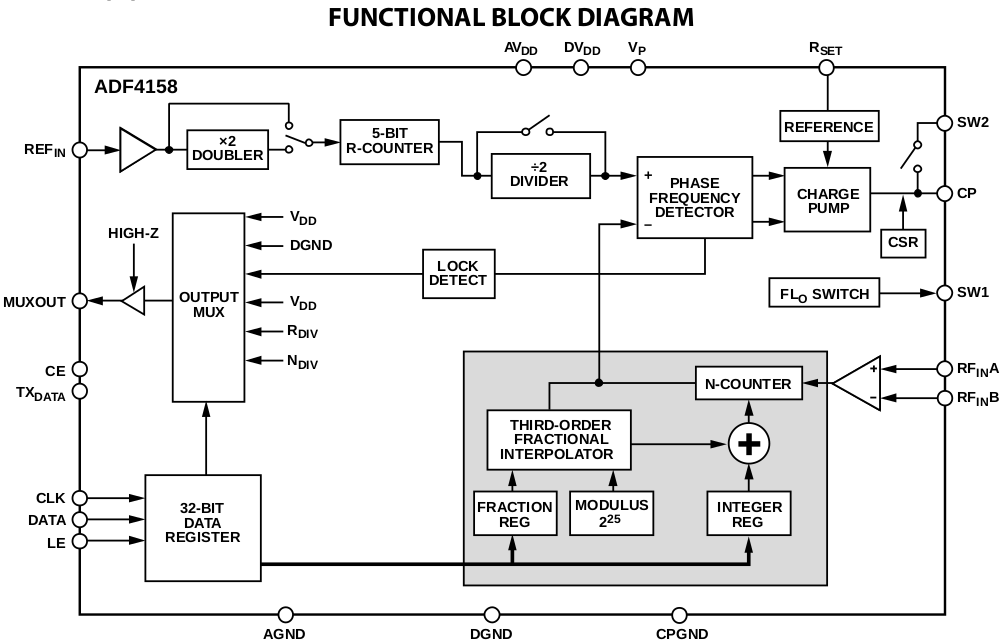
\includegraphics[width=0.75\textwidth]{data/adf4158-block-diagram.png}
        \caption{ADF4158 block diagram.}
        \label{fig:adf4158-block-diagram}
\end{figure}

The ADF4158 relies on an external VCO, described in \cref{sec:hmc431lp4rf}, whose output frequency
is given by Equation~\ref{eq:adf4158-rfout}. The output resolution is
$f_{\text{RES}} = f_{\text{PFD}}/2^{25}$ (see Equation~\ref{eq:adf4158-rfout} and its corresponding
parameter table for an explanation of $f_{\text{PFD}}$). The $2^{25}$ arises from the FRAC value
(set in registers 0 and 1) which is given 25 bits.

\begin{align}
  \text{RF}_{\text{OUT}} &= f_{\text{PFD}} \times \left(\text{INT} +
                           \left(\text{FRAC}/2^{25}\right)\right) \label{eq:adf4158-rfout} \\
  f_{\text{PFD}} &= \text{REF}_{\text{IN}} \times \left[\left(1 + D\right)/\left(R\times \left(1 +
                   T\right)\right) \right] \nonumber
\end{align}

\label{tab:adf4158-rfout-equation-vars}
\begin{tabularx}{\textwidth}{l X>{\raggedright\arraybackslash}X}
        \toprule
        \textbf{Parameter/Variable} & \textbf{Description} \\
        \midrule
        \endhead{}

        $\text{RF}_{\text{OUT}}$ & The VCO's output frequency. This is the frequency that's amplified for
        transmission. \\
        $f_{\text{PFD}}$ & The input frequency to the PFD post prescaling. In our case this is 20MHz. \\
        INT & The N counter that has a multiplicative effect on the VCO output frequency. \\
        FRAC & FRAC is the numerator of the fractional number added to INT. This is what distinguishes
        fractional-n synthesis from integer-n synthesis. It allows greater precision for the VCO
        output frequency without significantly increasing the prescalers and N counter. \\
        $\text{REF}_{\text{IN}} $ & The reference input frequency, which in our case is a 40MHz clock
        signal from the fanout buffer on the top level of the schematic. \\
        D & The doubler bit, which can be 0 or 1. If set to 1, the $\text{REF}_{\text{IN}}$ frequency is
        doubled before arriving at the R counter. \\
        R & The input prescaler. \\
        T & The divide- by-2 bit, which can be 0 or 1 and divides the frequency by 2 between the R
        prescaler and PFD. \\

        \bottomrule
\end{tabularx}

\subsubsection{Linked Sections}
\label{sec:adf4158-linked-sections}

\textit{\hyperref[sec:adf4158-pinout]{pinout}}

\subsubsection{Waveform Generation}
\label{sec:adf4158-waveform-generation}

The ADF4158 is capable of producing several different waveforms. The one used in this design is a
sawtooth ramp in frequency as a function of time, shown in
Figure~\ref{fig:adf4158-sawtooth-ramp}. There are 3 different parameters that determine the shape of
a ramp: (1) frequency deviation (the amount the frequency increases at each time step), (2) timeout
interval (the amount of time between each time step) and (3) the number of time steps. This is shown
diagrammatically in Figure~\ref{fig:adf4158-waveform-timing}. The equations governing these
parameters are given in Equation~\ref{eq:adf4158-waveform}. The number of steps is set directly in
register 6. In our configuration $f_{\text{DEV}} = 300\si{kHz}$ and $\text{Timer} = 0.5\si{\mu s}$,
which given that the number of steps is equal to 2000 and the starting frequency is 5.3GHz, the
sawtooth will ramp from 5.3GHz to 5.9GHz in 1ms. We also use a delay between bursts of
2ms. Equation~\ref{eq:adf4158-delay} is used to derive this.

\begin{align}
  f_{\text{DEV}} &= \left(f_{\text{PFD}}/2^{25}\right) \times \left(\text{DEV}\times
                   2^{\text{DEV\_OFFSET}}\right) \label{eq:adf4158-waveform} \\
  \text{Timer} &= \text{CLK}_1 \times \text{CLK}_2 \times \left(1/f_{\text{PFD}}\right) \nonumber
\end{align}

\label{tab:adf4158-waveform-equation-vars}
\begin{tabularx}{\textwidth}{l X>{\raggedright\arraybackslash}X}
        \toprule
        \textbf{Parameter/Variable} & \textbf{Description} \\
        \midrule

        $f_{\text{DEV}}$ & The frequency deviation for each frequency jump during ramp. \\
        $f_{\text{PFD}}$ & The input frequency to the PFD post prescaling. In our case this is 20MHz. \\
        DEV & A 16-bit value set in register 5. \\
        DEV\_OFFSET & A 4-bit word set in register 5. \\
        Timer & The time between each frequency hop. \\
        CLK\textsubscript{1} & A 12-bit clock divider set in register 2. \\
        CLK\textsubscript{2} & Another 12-bit clock divider set in register 4. \\

        \bottomrule
\end{tabularx}

\begin{equation}
        \label{eq:adf4158-delay}
        \text{Delay} = t_{\text{PFD}} \times \text{CLK}_1 \times \text{Delay Start Word}
\end{equation}

\label{tab:adf4158-delay-equation-vars}
\begin{tabularx}{\textwidth}{l X>{\raggedright\arraybackslash}X}
        \toprule
        \textbf{Parameter/Variable} & \textbf{Description} \\
        \midrule

        Delay & The delay between bursts. This is shown graphically in Figure~\ref{fig:adf4158-delay}. \\
        $f_{\text{PFD}}$ & The input frequency to the PFD post prescaling. In our case this is 20MHz. \\
        CLK\textsubscript{1} & A 12-bit clock divider set in register 2. \\
        Delay Start Word & A 12-bit value set in register 7. \\

        \bottomrule
\end{tabularx}

\begin{figure}[h]
        \centering
        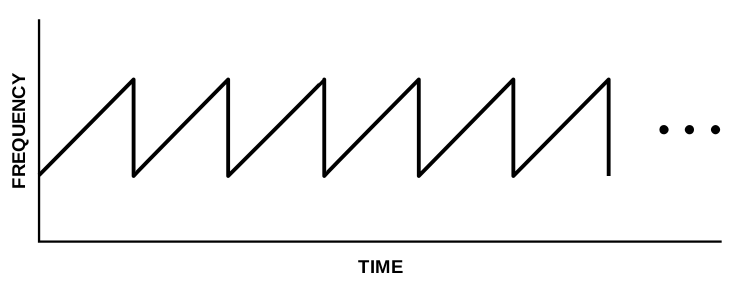
\includegraphics[width=0.5\textwidth]{data/adf4158-sawtooth-ramp.png}
        \caption{Sawtooth ramp.}
        \label{fig:adf4158-sawtooth-ramp}\end{figure}

\begin{figure}[h]
        \centering
        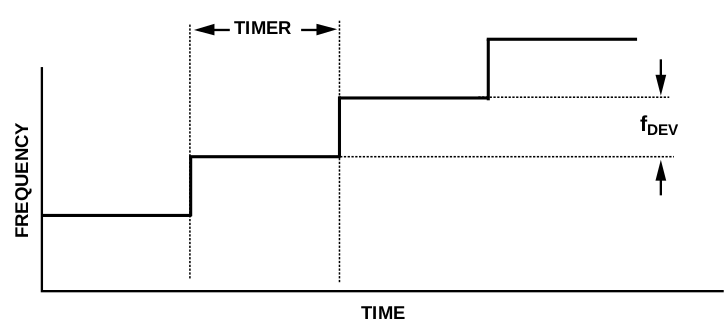
\includegraphics[width=0.5\textwidth]{data/adf4158-waveform-timing.png}
        \caption{Waveform timing.}
        \label{fig:adf4158-waveform-timing}
\end{figure}

\begin{figure}[h]
        \centering
        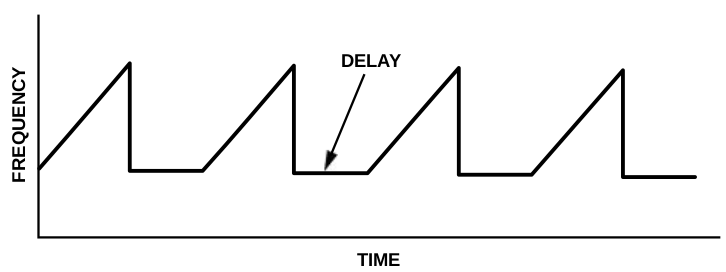
\includegraphics[width=0.5\textwidth]{data/adf4158-delay.png}
        \caption{Delay between ramps for sawtooth mode.}
        \label{fig:adf4158-delay}
\end{figure}

\begin{figure}[h]
        \centering
        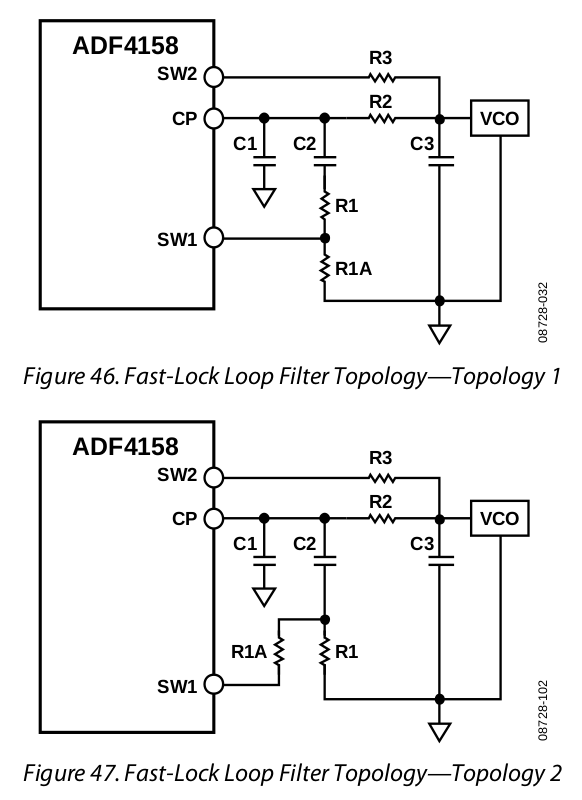
\includegraphics[width=0.5\textwidth]{data/adf4158-fast-lock.png}
        \caption{Fast lock topologies.}
        \label{fig:adf4158-fast-lock}
\end{figure}

\subsubsection{Configuration Registers}
\label{sec:adf4158-config-regs}

The ADF4158 contains 8 configuration registers. The configurations are shown in the tables
below. All reserved bits should be set to 0. The control bits are the least significant 3 bits of
each register and are set to the register number for each register (e.g.\ register 0 is 000 and
register 1 is 001). I've left these out of the tables because their values are obvious.

\label{tab:adf4158-reg-map-0}
\begin{tabularx}{\textwidth}{l l l X}
        \caption{FRAC/INT REGISTER (R0) MAP} \\
        \toprule
        Bit & Mnemonic & Value & Description \\
        \midrule

        3--14  & FRAC(MSB)      & 0   & This sets the 12 most significant bits of FRAC\@. We leave the
        fractional value at 0.                                               \\
        15--26 & INT            & 265 & This is the feedback, or N, counter. \\
        27--30 & MUXOUT Control & 15  & This enables ``readback to muxout'' which allows interrupting
        waveform generation and reading back the frequency at the time of interrupt. The
        functionality is not fully setup on the board(muxout connects to a DNP NMOS) and TX\_DATA,
        which can trigger the
        interrupt, is set to 0 by the FPGA HDL and left there.               \\
        31     & Ramp On        & 1   & This bit enables the ramp.           \\

        \bottomrule
\end{tabularx}

\label{tab:adf4158-reg-map-1}
\begin{tabularx}{\textwidth}{l l l X}
        \caption{LSB FRAC REGISTER(R1) MAP} \\
        \toprule
        Bit & Mnemonic & Value & Description \\
        \midrule

        3-14  & Reserved  & 0 & All reserved bits set to 0. \\
        15-27 & FRAC(LSB) & 0 & This sets the 13 least significant bits of FRAC\@. We leave the
        fractional value at 0.                              \\
        28-31 & Reserved  & 0 & All reserved bits set to 0. \\

        \bottomrule
\end{tabularx}

\label{tab:adf4158-reg-map-2}
\begin{tabularx}{\textwidth}{l l l X}
        \caption{R-DIVIDER REGISTER(R2) MAP} \\
        \toprule
        Bit & Mnemonic & Value & Description \\
        \midrule

        3--14  & CLK\textsubscript{1} Divider & 10 & One of the determinants of the duration of a
        time step in waveform generation. See \cref{sec:adf4158-waveform-generation} for more
        details.                                                                                                    \\
        15--19 & R-Counter                    & 1  & This 5-bit segment is used to divide the frequency of the reference
        signal
        before it enters the PFD\@. We leave it at 1 and thus do not use it to divide the frequency.                \\
        20     & Reference Doubler            & 0  & We leave this at 0 and thus do not use the doubler to double
        the reference signal frequency before input to the PFD\@. The maximum input frequency for
        the PFD is 30MHz and so doubling our 20MHz signal (we used the divider to divide the 40MHz
        signal by 2) would violate this condition.                                                                  \\
        21     & RDIV2                        & 1  & Inserts a divide-by-2 toggle flip-flop between the R-counter and
        PFD\@. This provides a 50\% duty cycle that allows cycle slip reduction to be used which
        improves lock times.                                                                                        \\
        22     & Prescaler                    & 1  & The prescaler limits the INT value and through that the maximum
        frequency to 3GHz. Since we have an INT value of 265 and our maximum frequency is almost
        double 3GHz we set this to 1.                                                                               \\
        23     & Reserved                     & 0  & All reserved bits set to 0.                                    \\
        24--27 & Charge Pump Current Setting  & 0  & Sets the current to the minimum value which is
        0.31mA and is the level necessary to use cycle slip reduction
        which we are.                                                                                               \\
        28     & CSR Enable                   & 1  & Enables cycle slip reduction which provides better lock times. \\
        29--31 & Reserved                     & 0  & All reserved bits are set to 0.                                \\

        \bottomrule
\end{tabularx}

\label{tab:adf4158-reg-map-3}
\begin{tabularx}{\textwidth}{l l l X}
        \caption{FUNCTION REGISTER(R3) MAP} \\
        \toprule
        Bit & Mnemonic & Value & Description \\
        \midrule

        3 & Counter Reset & 0 & When this is set to 1, the synthesizer counters are held in reset. For
        normal operation we set this to 0. \\
        4 & Charge Pump Three-State & 0 & Holds the charge pump in three-state mode if set to 1. For
        normal operation it must be set to 0. \\
        5 & Power-Down & 0 & Setting this to 1 powers down the device. Setting it to 0 allows normal
        operation. \\
        6 & PD Polarity & 1 & Set to 1 for positive VCO characteristics. Set to 0 for negative VCO
        characteristics. Since our VCO outputs a positive voltage signal we set this
        to 1. \\
        7 & LDP & 0 & Sets the minimum number of PFD cycles before a lock detect can be set. \\
        8 & FSK Enable & 0 & Disables FSK modulation. \\
        9 & PSK Enable & 0 & Disables PSK modulation. \\
        10-11 & Ramp Mode & 0 & Sets the waveform as a continuous sawtooth. \\
        12-13 & Reserved & 0 & All reserve bits are set to 0. \\
        14 & SD Reset & 0 & Setting this to 0 resets the $\Sigma-\Delta$ modulator on each write to
        register 0, which is the recommended operation. Setting this to 1 disables
        resetting the modulator. \\
        15 & N SEL & 0 & When set to 1, this creates an additional delay in setting INT and FRAC which can
        prevent the PLL overshooting. Since we set INT once and do not update it, this is
        not necessary and we leave it as 0. \\
        16-31 & Reserved & 0 & All reserve bits are set to 0. \\

        \bottomrule
\end{tabularx}

\label{tab:adf4158-reg-map-4}
\begin{tabularx}{\textwidth}{l l l X}
        \caption{TEST REGISTER(R4) MAP} \\
        \toprule
        Bit & Mnemonic & Value & Description \\
        \midrule

        3--6 & Reserved & 0 & All reserved bits are set to 0. \\
        7-18 & CLK\textsubscript{2} Divider & 1 & This is used to set the timeout interval in ramp
        generation. See
        \cref{sec:adf4158-waveform-generation}for more
        information. \\
        19-20 & CLK DIV Mode & 3 & This enables ramp divider mode, which specifies that
        CLK\textsubscript{1} and CLK\textsubscript{2} are used for ramp
        generation. \\
        21-22 & Readback to MUXOUT & 3 & Confusingly, this has been set to 3, which corresponds to neither
        of the supported values. Since we don't actually use the MUXOUT, this seems to be fine. If, at
        some point in the future, we do use the MUXOUT we will probably
        need to fix this. \\
        23-24 & Negative Bleed Current & 0 & This setting can help improve performance in the dead
        zone. We've disabled it. Note that this setting and readback
        to MUXOUT cannot simultaneously be enabled. To understand
        this setting better refer to \href{http://www.analog.com/media/en/technical-documentation/application-notes/AN-1154.pdf?doc=ADF4158.pdf}{AN-1154
          Application Note}. \\
        25 & Reserved & 0 & All reserved bits are set to 0. \\
        26-30 & $\Sigma-\Delta$ modulator mode & 0 & 0 enables this during normal operation. We can set it
        to 14 when FRAC=0. Even though we've set FRAC to 0,
        we have left this as 0 which seems strange. It
        shouldn't cause anything to malfunction, but may
        cause the ADF4158 to draw more power. We should
        experiment with setting this to 14 when using the
        actual board. \\
        31 & LE SEL & 0 & LE is the load enable pin which we use to load data onto the ADF4158's internal
        registers. Setting this to 0 enables the default operation of using the pin to
        set LE. Setting it to 1 would synchronize it with the reference signal. \\

        \bottomrule
\end{tabularx}

\label{tab:adf4158-reg-map-5}
\begin{tabularx}{\textwidth}{l l l X}
        \caption{DEVIATION REGISTER (R5) MAP} \\
        \toprule
        Bit & Mnemonic & Value & Description \\
        \midrule

        3--18 & Deviation Word & 31457 & This is used to set the size of successive frequency jumps during
        ramp. See \cref{sec:adf4158-waveform-generation} for more
        information. \\
        19--22 & Deviation Offset Word & 4 & This is also used to set the size of successive frequency
        jumps during ramp. See \cref{sec:adf4158-waveform-generation}
        for more information. \\
        23 & Deviation Select & 0 & Setting this bit to 1 is used for FSK as described on page 28 of the
        datasheet. Since we do not use FSK we leave this as 0. \\
        24 & Ramp 2 Enable & 0 & Setting this bit to 1 allows a second ramp with different settings than
        the first. We only need the first ramp. \\
        25 & FSK Ramp Enable & 0 & Setting this bit to 1 uses FSK. Again, we do not use FSK and so leave
        this bit as 0. \\
        26--27 & Interrupt & 0 & Sets the type of interrupt used to read the value of INT and FRAC of the
        ramp at a given moment. We don't read these values and therefore leave
        this as 0, which corresponds to interrupt off. \\
        28 & PAR Ramp & 0 & Setting this bit to 1 allows a parabolic ramp which we don't use. \\
        29 & Tx Ramp CLK & 0 & Setting this to 0 uses the clock divider (instead of the TX data clock) for
        clocking the ramp. \\
        30--31 & Reserved & 0 & \\

        \bottomrule
\end{tabularx}


\label{tab:adf4158-reg-map-6}
\begin{tabularx}{\textwidth}{l l l X}
        \caption{STEP REGISTER (R6) MAP} \\
        \toprule
        Bit & Mnemonic & Value & Description \\
        \midrule

        3--22 & Step Word & 2000 & This determines the number of steps in a ramp. To understand this see
        \cref{sec:adf4158-waveform-generation} on waveform generation. \\
        23 & Step SEL & 0 & This bit is used when 2 different ramps are needed (for instance with FSK). As
        we don't need this functionality we leave it off and set this bit to 0. \\
        24--31 & Reserved & 0 & \\

        \bottomrule
\end{tabularx}


\label{tab:adf4158-reg-map-7}
\begin{tabularx}{\textwidth}{l l l X}
        \caption{DELAY REGISTER (R7) MAP} \\
        \toprule
        Bit & Mnemonic & Value & Description \\
        \midrule

        3--14 & Delayed Start Word & 4000 & Sets the ramp start delay. We do not use a start delay, but we
        do use this to delay between ramps. \\
        15 & Delayed Start Enable & 0 & We do not use a start delay. \\
        16 & Delay Clock Select & 1 & Increases the period of the delay clock by multiplying the period of
        the PFD clock by CLK\textsubscript{1}. This creates an effective
        period of 500ns. \\
        17 & Ramp Delay & 1 & We enable a delay between ramp bursts. \\
        18 & Ramp Delay Fast Lock & 0 & Disables the ramp delay fast lock function. \\
        19--31 & Reserved & 0 & \\

        \bottomrule
\end{tabularx}

\subsubsection{Programming the Configuration Registers}
\label{sec:adf4158-program}

The write timing used to program the internal configuration registers is shown in
Fig.~\ref{fig:adf4158-write-timing}. The maximum clock frequency is $20 \si{MHz}$, which can be
achieved by dividing the reference clock frequency by 2. Additionally, LE must be brought low at
least half a clock period before data is clocked into the registers and held low for at least a
quarter of a period after the write ends. It then must be pulsed high for half a period before it
can be brought low again and another register write can occur. As shown in the diagram, the data is
sent MSB first and the last 3 bits are the control bits (which specify the destination register),
also sent MSB first. The registers must be configured in a specific order, detailed in the
``INITIALIZATION SEQUENCE'' section of the datasheet, and copied below for convenience.

\begin{enumerate}[noitemsep]
\item Delay register (R7)
\item Step register (R6)—load the step register (R6) twice, first with STEP SEL = 0 and then with
        STEP SEL = 1
\item Deviation register (R5)—load the deviation register (R5) twice, first with DEV SEL = 0 and
        then with DEV SEL = 1
\item Test register (R4)
\item Function register (R3)
\item R-divider register (R2)
\item LSB FRAC register (R1)
\item FRAC/INT register (R0)
\end{enumerate}

\begin{figure}[h]
        \centering
        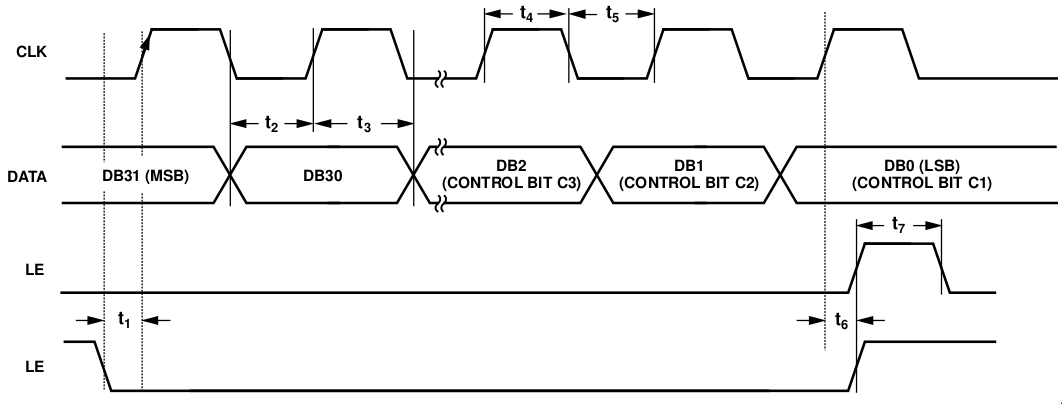
\includegraphics[width=0.75\textwidth]{data/adf4158-write-timing}
        \caption{ADF4158 write timing diagram.}
        \label{fig:adf4158-write-timing}
\end{figure}

\subsection{TLV172 Operational Amplifier}
\label{sec:tlv172-op-amp}

\subsubsection{Description}
\label{sec:tlv172-description}

The TLV172 op-amp is used to produce a gain of 2 to match the CP output of the ADF4158 to the VTUNE
input of the VCO\@. This is necessary since the charge pump supports a tune voltage of up to 5.5V
but the VCO has a tune range of 0V to 10V. A non-inverting amplifier configuration is used to
produce the necessary gain.

\subsubsection{Component Selection}
\label{sec:tlv172-component-selection}

The $100 \si{nF}$ bypass capacitor is recommended by the datasheet.

\subsubsection{PCB Layout}
\label{sec:tlv172-pcb}

The recommended layout for the TLV172 op amp is shown in Fig.~\ref{fig:tlv172-pcb}.

\begin{figure}[h]
        \centering
        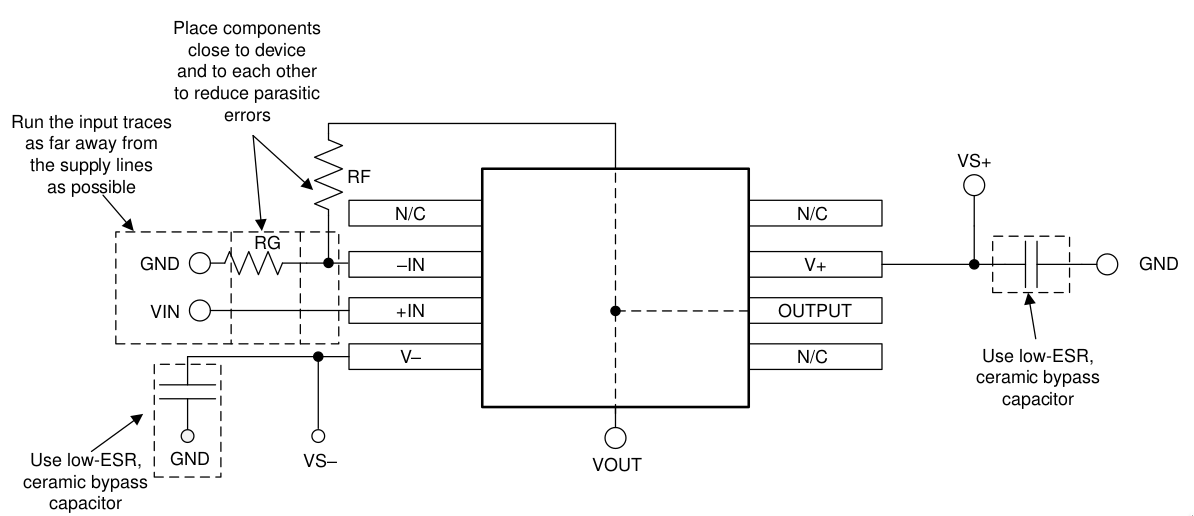
\includegraphics[width=\textwidth]{data/tlv172-pcb}
        \caption{TLV172 op-amp recommended PCB layout.}
        \label{fig:tlv172-pcb}
\end{figure}

\subsection{HMC431LP4RF VCO}
\label{sec:hmc431lp4rf}

The
\href{http://www.analog.com/media/en/technical_documentation/data_sheets/hmc431.pdf}{HMC431LP4RF} is
a radio-frequency VCO\@.

\subsection{DC4759J5020AHF Directional Coupler}
\label{sec:dc4759j5020ahf}

\subsubsection{Description}
\label{sec:dc4759j5020ahf-description}

The DC4759J5020AHF is a directional coupler with a $20 \si{dB}$ coupling factor, $0.17 \si{dB}$
insertion loss and $10.3 \si{dB}$ directivity. It is used to redirect some of the transmission power
back to the \hyperref[sec:adl5802]{mixer}'s local oscillator input. A directional coupler is a
4-terminal device, whose general form is shown in Fig.~\ref{fig:directional-coupler}. The coupling
factor gives the amount of input power that is redirected to the coupled port, the insertion loss
gives the amount of input power that is transmitted through to the output port and the directivity
is a measure of the coupler's ability to isolate the coupled and isolation ports. The actual
equations are given in Eq.~\ref{eq:coupling-factor}, Eq.~\ref{eq:insertion-loss} and
Eq.~\ref{eq:directivity}. In an ideal coupler, all input power is either transmitted through or
coupled. However, in all real directional couplers, some power is directed to the isolation port. In
our case $25.8 \si{dBm}$ is directed for transmission, $6 \si{dBm}$ is coupled, and $-4.3 \si{dBm}$
is sent to the isolated port.

\begin{figure}[h]
        \centering
        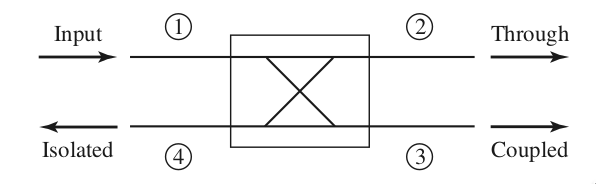
\includegraphics[width=0.5\textwidth]{data/directional-coupler}
        \caption{Directional coupler.}
        \label{fig:directional-coupler}
\end{figure}

\begin{equation}
        \label{eq:coupling-factor}
        C = 10 \log \frac{P_1}{P_3}
\end{equation}

\begin{equation}
        \label{eq:insertion-loss}
        L = 10 \log \frac{P_1}{P_2}
\end{equation}

\begin{equation}
        \label{eq:directivity}
        D = 10 \log \frac{P_3}{P_4}
\end{equation}

\subsubsection{PCB Layout}
\label{sec:dc4759j5020ahf-pcb}

The recommended PCB layout is shown in Fig.~\ref{fig:dc4759j5020ahf-pcb}, where the leftmost pads
correspond to the input and direct pins. All PCB traces leading from the pads should have a $50
\si{\Omega}$ characteristic impedance.

\begin{figure}[h]
        \centering
        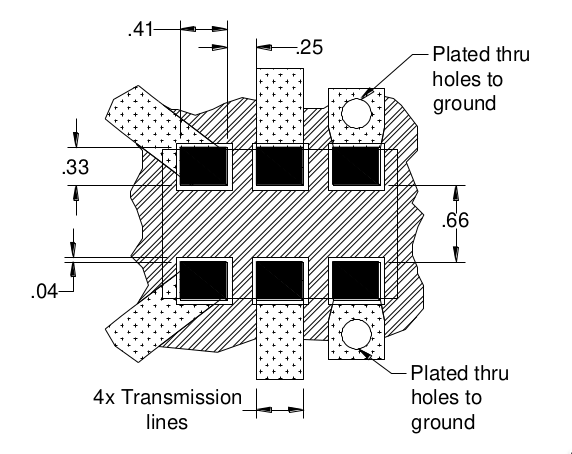
\includegraphics[width=0.3\textwidth]{data/dc4759j5020ahf-pcb}
        \caption{DC4759J5020AHF recommended PCB layout.}
        \label{fig:dc4759j5020ahf-pcb}
\end{figure}

\subsection{PD4859J5050S2HF Wilkinson Power Divider}
\label{sec:pd4859j5050s2hf}

\subsubsection{Description}
\label{sec:pd4859j5050s2hf-description}

The PD4859J5050S2HF is a Wilkinson power divider that equally divides the input power between the
two output ports. We use one after the \hyperref[sec:hmc431lp4rf]{VCO} to share its $2 \si{dBm}$
output power between the \hyperref[sec:se2567l]{power amplifier} and the RF\textsubscript{IN} port
of the \hyperref[sec:adf4158]{frequency synthesizer}.

\subsubsection{PCB Layout}
\label{sec:pd4859j50502shf-pcb}

The recommended layout is shown in Fig.~\ref{fig:pd4859j50502shf-pcb}. Ensure the location of the
external $100 \si{\Omega}$ 0603 resistor matches the location shown in the figure. All ports have a
$50 \si{\Omega}$ characteristic impedance which must be matched by the input and output traces.

\begin{figure}[h]
        \centering
        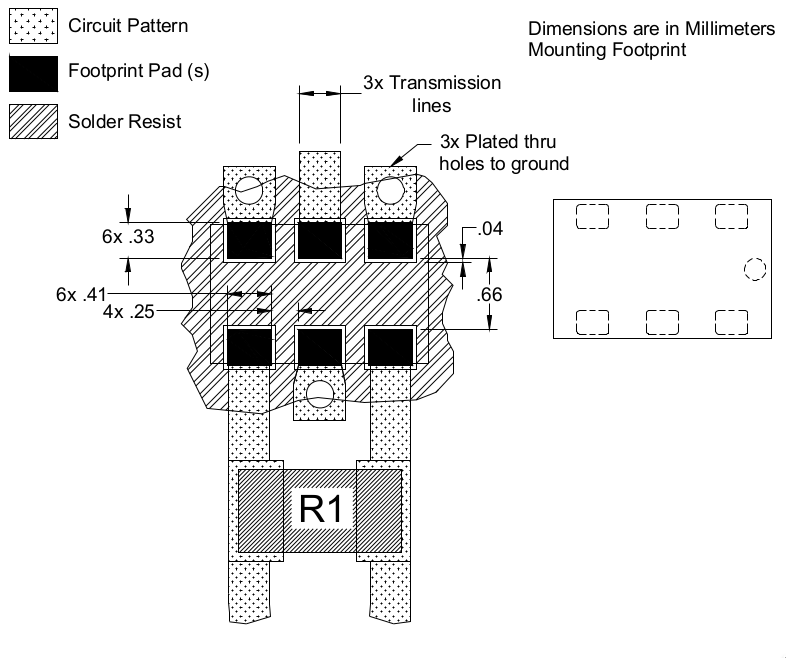
\includegraphics[width=0.5\textwidth]{data/pd4859j50502shf-pcb}
        \caption{PD4859J50502SHF recommended PCB layout. Note the location of the resistor.}
        \label{fig:pd4859j50502shf-pcb}
\end{figure}

\subsection{PAT1220 RF Attenuator}
\label{sec:pat1220}

\subsubsection{Description}
\label{sec:pat1220-description}

The PAT1220 is a simple resistive attenuator that can be used to preserve the shape of a signal but
decrease its power.

We use a $5 \si{dB}$ attenuator between the \hyperref[sec:hmc431lp4rf]{VCO} and
\hyperref[sec:se2567l]{power amplifier} in order to set the power amplifier's output power to its
typical value of $26 \si{dBm}$ as specified by the datasheet (it has a small-signal gain of
$32 \si{dB}$). This is enough power for a small radar (see~\cref{sec:distance}) and is sufficiently
below the $1 \si{dB}$ compression point, which should ensure good linearity.

I've placed a $3 \si{dB}$ attenuator between one of the \hyperref[sec:pd4859j5050s2hf]{Wilkinson
  power divider} outputs and the RF\textsubscript{IN} port of the \hyperref[sec:adf4158]{frequency
  synthesizer}. This shouldn't be strictly necessary, since the max power of the
RF\textsubscript{IN} port is $0 \si{dBm}$. However, using $-1 \si{dBm}$ would be playing it a bit
close. Additionally, the $2 \si{dBm}$ output of the VCO is a typical power output, not the max
power, which makes foregoing the attenuator even more dangerous. Finally, the RF\textsubscript{IN}
port supports an input power of as low as $-10 \si{dBm}$, so we have plenty of room on the downside.

The last attenuator ($6 \si{dB}$) is used at the coupled port of the
\hyperref[sec:dc4759j5020ahf]{directional coupler}, on its way to the local oscillator input of the
\hyperref[sec:adl5802]{mixer}. Again, the unattenuated $6 \si{dBm}$ should be ok (the max input
power of the LO is $10 \si{dBm}$). However, using the attenuator brings the LO power down to the
typical value specified by the mixer datasheet. To make sure our devices operate properly, we might
as well use the conditions recommended by the datasheet.

\subsubsection{PCB Layout}
\label{sec:pat1220-pcb-layout}

The recommended layout is shown in Fig.~\ref{fig:pat1220-pcb}. The ports are matched for a $50
\si{\Omega}$ characteristic trace impedance.

\begin{figure}[h]
        \centering
        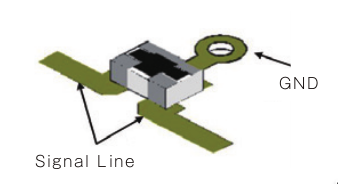
\includegraphics[width=0.25\textwidth]{data/pat1220-pcb}
        \caption{PAT1220 recommended PCB layout.}
        \label{fig:pat1220-pcb}
\end{figure}

\subsection{SE2567L Power Amplifier}
\label{sec:se2567l-power-amp}


%%% Local Variables:
%%% mode: latex
%%% TeX-master: "fmcw-radar"
%%% End:
